
%(BEGIN_QUESTION)
% Copyright 2014, Tony R. Kuphaldt, released under the Creative Commons Attribution License (v 1.0)
% This means you may do almost anything with this work of mine, so long as you give me proper credit

Et retningsbestemt overstrømsrelé av typen General Electric modell IBC er koblet til en strømtransformator med følgende kretsverdier. Merk spesielt $R$- og $X_L$-verdiene inne i CT-en, som representerer henholdsvis sekundærviklingsresistans og lekkinduktans:

$$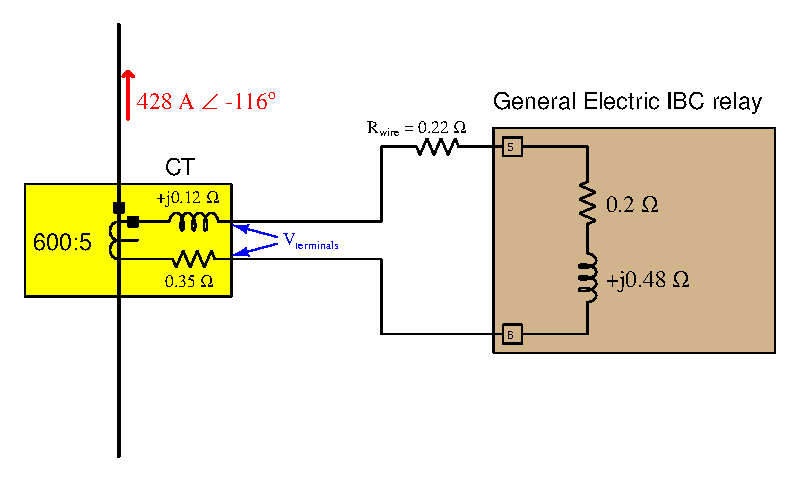
\includegraphics[width=15.5cm]{i00829x01.eps}$$

Beregn strømmen i CT-sekundærkretsen og spenningen ut fra CT-en, forutsatt ideelt strømforhold 600:5:

\vskip 10pt

$I_{sec} = $ \underbar{\hskip 50pt}

\vskip 10pt

$V_{terminals} = $ \underbar{\hskip 50pt}

\vskip 20pt \vbox{\hrule \hbox{\strut \vrule{} {\bf Forslag til sokratisk diskusjon} \vrule} \hrule}

\begin{itemize}
\item{} Beregn nødvendig C-klasse for denne CT-en for å unngå uakseptabel feil ved feilstrøm, forutsatt maksimal feilstrøm på 9 kA.
\end{itemize}

\underbar{file i00829}
%(END_QUESTION)





%(BEGIN_ANSWER)

$I_{sec} = $ \underbar{3.56667 A $\angle$ $-116^o$}

\vskip 10pt

$V_{terminals} = $ \underbar{2.275 V $\angle$ $-67.19^o$}

\vskip 10pt

Hvis du forsøker å beregne terminalspenning ($V_{terminals}$) ved å multiplisere strøm og CT-viklingsimpedans ([3.56667 A $\angle$ $-116^o$] $\times$ [0.35 $\Omega$ + j0.12 $\Omega$]), gjør du en alvorlig feil. Denne beregningen gir spenningsfallet {\it over viklingsimpedansen}, ikke spenningen mellom CT-terminalene. Husk at CT-viklingen er eneste kilde i sekundærkretsen, alt annet i kretsen er last.

%(END_ANSWER)





%(BEGIN_NOTES)

Sekundærstrømmen blir ganske enkelt $5 \over 600$ av primærstrømmen (kraftlinjestrømmen), uten faseforskyvning. Husk at en CT oppfører seg som en {\it strømkilde}, og vil ideelt levere korrekt strøm uavhengig av burden.

\vskip 10pt

$V_{terminals}$ er lik kretsstrøm multiplisert med total impedans i ledere og relé (total burden) ($V = IZ$):

$$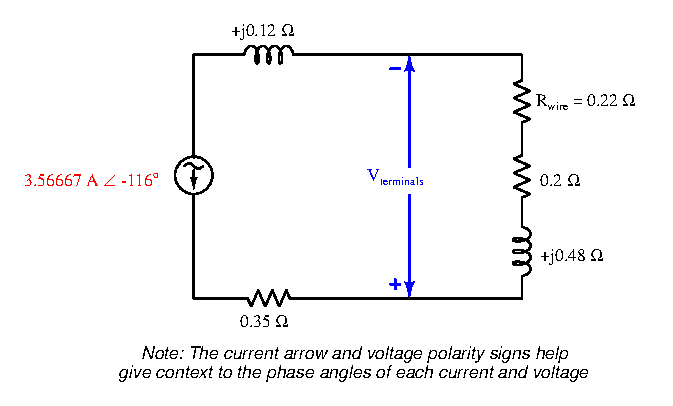
\includegraphics[width=15.5cm]{i00829x02.eps}$$

$$Z_{burden} = (0.22 + j0 \> \Omega) + (0.2 + j0 \> \Omega) + (0 + j0.48 \> \Omega)$$

$$Z_{burden} = 0.42 + j0.48 \> \Omega = 0.6378 \> \Omega \angle 48.81^o$$

\vskip 10pt

$$V_{terminals} = I Z_{burden}$$

$$V_{terminals} = (3.56667 \hbox{ A} \angle -116^o) (0.6378 \> \Omega \angle 48.81^o)$$

$$V_{terminals} = 2.275 \hbox{ V} \angle -67.19^o$$

%INDEX% Electronics review: 3-phase voltage/current/power calculation
%INDEX% Electronics review: AC reactance and impedance
%INDEX% Electronics review, phasor expressions of circuit quantities
%INDEX% Electronics review: series and parallel AC circuits

%(END_NOTES)
